\documentclass{standalone}
\usepackage{tikz}
\usepackage{ctex,siunitx}
\setCJKmainfont{Noto Serif CJK SC}
\usepackage{tkz-euclide}
\usepackage{amsmath}
\usepackage{wasysym}
\usetikzlibrary{patterns, calc}
\usetikzlibrary {decorations.pathmorphing, decorations.pathreplacing, decorations.shapes,}
\begin{document}
\small
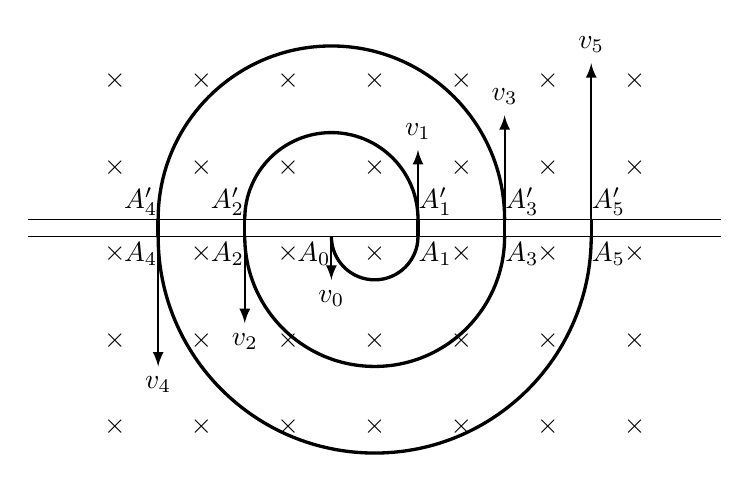
\begin{tikzpicture}[>=latex,scale=1.1]
  \foreach \x in {1,...,7}
  \foreach \y in {1,...,5}
  {
      \node at (\x,\y){$\times$};
  }
  
  \draw (0,3.2)--(8,3.2);
  \draw (0,3.4)--(8,3.4);
  
  \draw[very thick] (3.5,3.2) arc (180:360:.5);  
  \draw[->, thick]  (3.5,3.2)--(3.5,3.2-.5)node[below]{$v_0$};
  \draw[very thick] (3.5+1,3.2)--(3.5+1,3.2+.2);
  \draw[very thick] (3.5+1,3.2+.2) arc (0:180:1);  
  \draw[->, thick]  (3.5+1,3.2+.2)--(3.5+1,3.2+.2+.8)node[above]{$v_1$};
  \draw[very thick] (3.5-1,3.2+.2)--(3.5-1,3.2);
  \draw[very thick] (3.5-1,3.2) arc  (180:360:1.5);  
  \draw[->, thick]  (3.5-1,3.2)--(3.5-1,3.2-1)node[below]{$v_2$};
  \draw[very thick] (3.5+2,3.2)--(3.5+2,3.2+.2);
  \draw[very thick] (3.5+2,3.2+.2) arc  (0:180:2);  
  \draw[->, thick]  (3.5+2,3.2+.2)--(3.5+2,3.2+.2+1.2)node[above]{$v_3$};
  \draw[very thick] (3.5-2,3.2+.2)--(3.5-2,3.2);
  \draw[very thick] (3.5-2,3.2) arc  (180:360:2.5);  
  \draw[->, thick]  (3.5-2,3.2)--(3.5-2,3.2-1.5)node[below]{$v_4$};
  \draw[very thick] (3.5-2+5,3.2)--(3.5-2+5,3.2+.2);
  \draw[->, thick]  (3.5-2+5,3.2+.2)--(3.5-2+5,3.2+.2+1.8)node[above]{$v_5$};
  
  \node at (3.5-.2,3){$A_0$};
  \node at (4.5+.2,3){$A_1$};
  \node at (2.5-.2,3){$A_2$};
  \node at (5.5+.2,3){$A_3$};
  \node at (1.5-.2,3){$A_4$};
  \node at (6.5+.2,3){$A_5$};
  
  \node at (4.5+.2,3.6){$A'_1$};
  \node at (2.5-.2,3.6){$A'_2$};
  \node at (5.5+.2,3.6){$A'_3$};
  \node at (1.5-.2,3.6){$A'_4$};
  \node at (6.5+.2,3.6){$A'_5$};
\end{tikzpicture}
\end{document}